\section{边界模式}
\label{sec:wave-modes}

弦总有端点，波跑到端点后会怎样？半直线上用反射就能回答，有界区间上波来回反射，解的结构要用模式描述。边界条件决定可用的模式，这一点和第~\ref{chap:diffusion-equations}章相同，时间因子却完全不同。

\paragraph{半直线：固定端的翻转反射}
考虑$x>0$上的弦，端点$x=0$固定。d'Alembert公式需要整条实轴上的数据，我们把初值延拓到$x<0$上，让解自动在$x=0$处为零。如果实轴上的数据关于原点是奇函数，解也是奇函数，因为$-u(-x,t)$满足同样的问题，由唯一性等于$u$；奇函数在$0$处的值只能是$0$。

于是对$u_0,u_1$作\term{奇延拓}（odd extension）：$x<0$时令$u_0(x)=-u_0(-x)$，$u_1(x)=-u_1(-x)$。这是在墙的另一侧放一个翻转的镜像。把延拓后的数据代入式~\eqref{eq:wave-dalembert}，分情况计算。当$x\geq ct$时，$x-ct\geq0$，用不到延拓，公式不变。当$0\leq x<ct$时，$u_0(x-ct)=-u_0(ct-x)$，积分中$(x-ct,\,ct-x)$是对称区间，奇函数的积分为零。

这样就得到半直线固定端的解：
\begin{equation}
 u(x,t)=
 \begin{cases}
  \dfrac12\bigl[u_0(x-ct)+u_0(x+ct)\bigr]+\dfrac1{2c}\displaystyle\int_{x-ct}^{x+ct}u_1\,\mathrm{d}s, & x\geq ct,\\
  \dfrac12\bigl[u_0(ct+x)-u_0(ct-x)\bigr]+\dfrac1{2c}\displaystyle\int_{ct-x}^{ct+x}u_1\,\mathrm{d}s, & 0\leq x<ct .
 \end{cases}
 \label{eq:wave-halfline-fixed}
\end{equation}
第二行中，$-\frac12u_0(ct-x)$是从左侧镜像传来的、已经翻转的反射波。

\paragraph{半直线：自由端的同号反射}
自由端要求$\partial_xu(0,t)=0$。偶函数的导数在$0$处为零，所以改作\term{偶延拓}（even extension）：$u_0(-x)=u_0(x)$，$u_1(-x)=u_1(x)$。镜像不翻转。同样的计算在$0\leq x<ct$时给出
\begin{equation}
 u(x,t)=\frac12\bigl[u_0(ct+x)+u_0(ct-x)\bigr]+\frac1{2c}\Bigl[\int_0^{ct+x}u_1\,\mathrm{d}s+\int_0^{ct-x}u_1\,\mathrm{d}s\Bigr],
 \label{eq:wave-halfline-free}
\end{equation}
$x\geq ct$时仍是式~\eqref{eq:wave-dalembert}。

这两个公式要成为$C^{2}$解，延拓后的数据必须足够光滑。固定端要求$u_0(0)=u_0''(0)=u_1(0)=0$，这正是表~\ref{tab:wave-boundary}之后的相容条件在$g\equiv0$、$f\equiv0$时的结果。自由端要求$u_0'(0)=u_1'(0)=0$。解也是唯一的：若$u$是半直线上固定端的$C^{2}$解，由方程得$\partial_x^{2}u(0,t)=c^{-2}\partial_t^{2}u(0,t)=0$，它的奇延拓在实轴上是$C^{2}$解，再用定理~\ref{thm:wave-dalembert}；自由端用偶延拓同理。

\paragraph{走一遍反射}
取$c=1$，$u_1=0$，初始位移是中心在$x=3$的帐篷$\Lambda(x-3)$。它分成两半，右行的一半直接走开，左行的一半$\frac12\Lambda(x-3+t)$在$t=2$时到达端点，$t=3$时中心位于端点。

在反射发生的时刻，两种端点表现最为不同。取$t=3$，靠近端点$0\leq x\leq1$处的解由式~\eqref{eq:wave-halfline-fixed}和式~\eqref{eq:wave-halfline-free}算出：
\[
 u^{\mathrm{fix}}(x,3)=\tfrac12[\Lambda(x)-\Lambda(-x)]=0,\qquad u^{\mathrm{free}}(x,3)=\Lambda(x).
\]
固定端附近入射波和镜像恰好抵消，位移为零，能量此时全在速度里；自由端附近两者相加，端点位移翻倍，高度达到$1$。

反射之后再取一点比较。在$(x,t)=(1,\,7/2)$处，$ct+x=9/2$，$ct-x=5/2$，代入两个公式：
\[
 u^{\mathrm{fix}}(1,\tfrac72)=\tfrac12[\Lambda(\tfrac32)-\Lambda(-\tfrac12)]=-\tfrac14,\qquad u^{\mathrm{free}}(1,\tfrac72)=\tfrac14 .
\]
固定端反射回来的波被翻转，自由端反射回来的波保持同号，如图~\ref{fig:wave-reflection}。

\begin{BookInlineFigure}
  \centering
  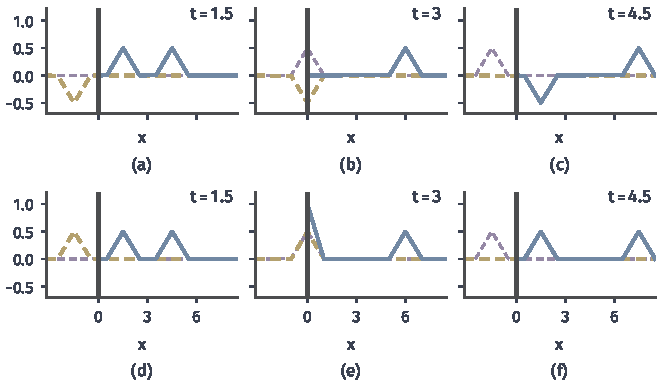
\includegraphics[width=112mm]{figures/06-differential-equations/02-partial-differential-equations/matplotlib/wave-reflection/figure.pdf}
  \caption{半直线上$\Lambda(x-3)$的两半波在端点（深灰竖线）的反射，$c=1$。上排是固定端，下排是自由端。紫色虚线是左行的入射波，黄色虚线是从$x<0$一侧传来的镜像，上排翻转，下排不翻转。蓝线是$x\geq0$上的解，等于两者与右行波之和。}
  \label{fig:wave-reflection}
\end{BookInlineFigure}

\paragraph{区间：分离变量}
现在考虑$(0,L)$上的弦。波在两端之间来回反射，用镜像可以写出来，但更好的办法是换一个角度：寻找形状不变、只有幅度随时间变化的解。设$u(x,t)=X(x)\Theta(t)$，代入$\partial_t^{2}u=c^{2}\partial_x^{2}u$并除以$c^{2}X\Theta$，得到
\[
 \frac{\ddot{\Theta}(t)}{c^{2}\Theta(t)}=\frac{X''(x)}{X(x)}.
\]

左边只依赖$t$，右边只依赖$x$，所以两边等于同一个常数，记作$-\lambda$。这种做法称为\term{分离变量法}（separation of variables）。空间部分是特征值问题，时间部分是简谐振子：
\begin{equation}
 -X''=\lambda X,\qquad \ddot{\Theta}=-c^{2}\lambda\,\Theta .
 \label{eq:wave-separation}
\end{equation}

边界条件落在$X$上。先看两端固定的情形，$X(0)=X(L)=0$。把$X$乘上式并积分，分部积分后边界项为零：
\[
 \lambda\int_0^{L}X^{2}\,\mathrm{d}x=\int_0^{L}(X')^{2}\,\mathrm{d}x .
\]
非零的$X$不可能是常数（它要在端点取零），所以$\lambda>0$。记$\lambda=k^{2}$，$k>0$，通解是$X=A\cos kx+B\sin kx$。条件$X(0)=0$给出$A=0$，条件$X(L)=0$给出$\sin kL=0$，于是
\begin{equation}
 k_n=\frac{n\pi}{L},\qquad X_n(x)=\sin\frac{n\pi x}{L},\qquad n=1,2,\ldots
 \label{eq:wave-dirichlet-modes}
\end{equation}

时间部分的频率是$\omega_n=ck_n=cn\pi/L$，称为第$n$个\term{固有频率}（natural frequency）。

其他端点组合做同样的计算，只是条件换了，结果列在表~\ref{tab:wave-modes}中，前三个模式画在图~\ref{fig:wave-mode-shapes}中。两端自由时多出$\lambda=0$的常数模式，它的时间因子是$a+bt$：整根弦没有受到任何拉回的力，可以整体匀速平移。一端固定一端自由时，$X$在固定端为零、在自由端斜率为零，波长的四分之一装进弦长，所以$k$是$\pi/(2L)$的奇数倍。

\begin{BookInlineTable}
  \centering
  \caption{区间$(0,L)$上三种端点组合的空间模式}
  \label{tab:wave-modes}
  \begin{tabular}{lll}
    \toprule
    端点 & $X_n$ & $k_n$\\
    \midrule
    固定--固定 & $\sin(n\pi x/L)$ & $n\pi/L$，$n\geq1$\\
    自由--自由 & $\cos(n\pi x/L)$ & $n\pi/L$，$n\geq0$\\
    固定--自由 & $\sin((n-\tfrac12)\pi x/L)$ & $(n-\tfrac12)\pi/L$，$n\geq1$\\
    \bottomrule
  \end{tabular}
\end{BookInlineTable}

\begin{BookInlineFigure}
  \centering
  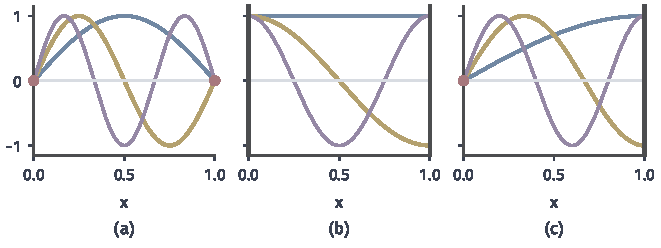
\includegraphics[width=112mm]{figures/06-differential-equations/02-partial-differential-equations/matplotlib/wave-mode-shapes/figure.pdf}
  \caption{$L=1$时的前三个空间模式，蓝、黄、紫依次为$n$增大。红点表示固定端（$X=0$），深灰粗竖线表示自由端（$X'=0$）。(a)固定--固定。(b)自由--自由，蓝线是常数模式。(c)固定--自由。}
  \label{fig:wave-mode-shapes}
\end{BookInlineFigure}

\paragraph{模式展开的解}
两端固定时，由式~\eqref{eq:wave-separation}和线性性，把所有模式叠加起来。把初值按$\sin(n\pi x/L)$展开，系数是
\begin{equation}
 a_n=\frac2L\int_0^{L}u_0(x)\sin\frac{n\pi x}{L}\,\mathrm{d}x,\qquad b_n=\frac2L\int_0^{L}u_1(x)\sin\frac{n\pi x}{L}\,\mathrm{d}x .
 \label{eq:wave-coefficients}
\end{equation}
这组正弦函数在$L^{2}(0,L)$中正交而且完备，这是Fourier级数理论的结果，可参考\BookChapterRef{chap:fourier-transform}{卷四第14章“Fourier变换”}。下面的定理说明，数据足够光滑时级数给出经典解。

\begin{theorem}[两端固定的模式解]
\label{thm:wave-series}
设$u_0\in C^{3}[0,L]$，$u_1\in C^{2}[0,L]$，并满足在$x=0,L$处$u_0=u_0''=0$，$u_1=0$。记$\omega_n=cn\pi/L$，系数由式~\eqref{eq:wave-coefficients}给出，则
\begin{equation}
 u(x,t)=\sum_{n=1}^{\infty}\Bigl(a_n\cos\omega_nt+\frac{b_n}{\omega_n}\sin\omega_nt\Bigr)\sin\frac{n\pi x}{L}
 \label{eq:wave-series}
\end{equation}
是$[0,L]\times[0,\infty)$上的$C^{2}$函数，满足$\partial_t^{2}u=c^{2}\partial_x^{2}u$、两端为零和两个初始条件。
\end{theorem}

\begin{proof}
关键是系数衰减得足够快，使逐项求两次导后的级数一致收敛。记$k_n=n\pi/L$。对$a_n$的积分分部三次：前两次的边界项因$u_0$和$u_0''$在端点为零而消失，第三次仍保留积分。于是
\[
 a_n=-\frac{1}{k_n^{3}}\cdot\frac2L\int_0^{L}u_0'''(x)\cos k_nx\,\mathrm{d}x .
\]

右端的积分是$u_0'''$关于余弦系的系数，由Bessel不等式，这些系数平方可和，所以$(n^{3}a_n)$属于$\ell^{2}$。同样对$b_n$分部两次，$(n^{2}b_n)$属于$\ell^{2}$。由Cauchy--Schwarz不等式，
\[
 \sum_{n}n^{2}\lvert a_n\rvert=\sum_{n}\frac{n^{3}\lvert a_n\rvert}{n}\leq\Bigl(\sum_{n}n^{6}a_n^{2}\Bigr)^{1/2}\Bigl(\sum_{n}\frac1{n^{2}}\Bigr)^{1/2}<\infty,
\]
同理$\sum_nn\lvert b_n\rvert<\infty$。

式~\eqref{eq:wave-series}的通项及其对$x,t$的至多二阶偏导，绝对值都不超过常数乘$n^{2}\lvert a_n\rvert+n\lvert b_n\rvert$。由Weierstrass判别法，这些级数都一致收敛，可以逐项求导，所以$u$是$C^{2}$函数。每一项都满足方程和边界条件，因而$u$也满足。令$t=0$，由余弦和正弦展开的收敛性，得到两个初始条件。
\end{proof}

式~\eqref{eq:wave-series}的解也是唯一的，这要等第~\ref{sec:wave-energy}节用能量证明。数据不够光滑时，只要$(u_0,u_1)\in H_0^{1}(0,L)\times L^{2}(0,L)$，级数仍在能量的意义下收敛，所得的函数是弱解，折线初值就属于这种情形。

自由端的常数模式可以手算验证。取$L=1$，$c=1$，两端自由，$u_0=0$，$u_1=1+\cos\pi x$。把$u_1$看成常数模式和第一个余弦模式之和，常数模式的时间因子是$t$，第一个模式的时间因子是$\sin(\pi t)/\pi$，所以
\[
 u(x,t)=t+\frac{\sin\pi t}{\pi}\cos\pi x .
\]
代入可得
\[
 \partial_t^{2}u=-\pi\sin(\pi t)\cos\pi x=\partial_x^{2}u .
\]
两端$\partial_xu=0$，$t=0$时位移为零，速度是$u_1$。第一项让弦整体匀速上升，第二项是叠加在上面的振动，这是固定端不会出现的现象。

\paragraph{驻波是两列行波之和}
式~\eqref{eq:wave-series}的每一项称为\term{驻波}（standing wave）：形状不变，只是幅度随时间振荡，节点永远不动。这看起来和行波毫无关系。其实由积化和差，
\begin{equation}
 \cos(ckt)\sin(kx)=\frac12\bigl[\sin k(x-ct)+\sin k(x+ct)\bigr].
 \label{eq:wave-standing}
\end{equation}

一个驻波就是一列右行波和一列左行波的叠加，这正是式~\eqref{eq:wave-general-solution}的形式。两列波不断反射，在区间内干涉出固定的形状。图~\ref{fig:wave-standing-traveling}用$L=1$，$c=1$，$n=1$画出了这个分解。

\begin{BookInlineFigure}
  \centering
  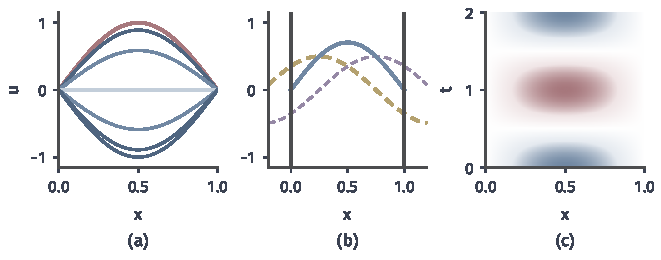
\includegraphics[width=112mm]{figures/06-differential-equations/02-partial-differential-equations/matplotlib/wave-standing-traveling/figure.pdf}
  \caption{第一个驻波$\cos(\pi t)\sin(\pi x)$，$L=1$，$c=1$。(a)不同时刻的形状，红色是$t=0$，端点始终为零。(b)$t=0.25$的分解：黄色虚线是左行波，紫色虚线是右行波，蓝线是两者之和，它在两端（深灰竖线）为零。(c)时空热图，蓝为正，红为负，$t=1$附近弦完全翻转。}
  \label{fig:wave-standing-traveling}
\end{BookInlineFigure}

把这个观察用到整个级数上。对式~\eqref{eq:wave-series}逐项用式~\eqref{eq:wave-standing}，并把$u_0,u_1$作奇延拓后再以$2L$为周期延拓到实轴，得到的正是d'Alembert公式
\begin{equation}
 u(x,t)=\frac12\bigl[\tilde{u}_0(x-ct)+\tilde{u}_0(x+ct)\bigr]+\frac1{2c}\int_{x-ct}^{x+ct}\tilde{u}_1(s)\,\mathrm{d}s .
 \label{eq:wave-interval-extension}
\end{equation}
其中$\tilde{u}_0,\tilde{u}_1$是延拓后的函数。奇延拓保证$x=0$处为零，以$2L$为周期再关于$x=L$也是奇的，所以$x=L$处也为零。这就是在两堵墙之间反复照镜子：反射和模式是同一个解的两种写法。式~\eqref{eq:wave-interval-extension}说明解沿时间有周期$2L/c$，一个波跑到对端再回来刚好用这么长时间。

\paragraph{手算：拨弦的模式}
取$L=1$，$c=1$，初速度为零，把中点拉起成折线$u_0=\min\{x,1-x\}$。由式~\eqref{eq:wave-coefficients}，分部积分后，正弦系数是
\begin{equation}
 a_n=\frac{4}{n^{2}\pi^{2}}\sin\frac{n\pi}{2}.
 \label{eq:wave-pluck-coefficients}
\end{equation}
$n$为偶数时$a_n=0$，这是因为折线关于中点对称，而偶数模式关于中点反对称。前三个非零系数是
\[
 a_1=\frac4{\pi^{2}}\approx0.405,\qquad a_3=-\frac4{9\pi^{2}}\approx-0.045,\qquad a_5=\frac4{25\pi^{2}}\approx0.016 .
\]

解是$u=\sum_na_n\cos(n\pi t)\sin(n\pi x)$。我们用两个时刻核对。在$t=1/2$、$x=1/2$处，奇数$n$的$\cos(n\pi/2)=0$，所以$u(\frac12,\frac12)=0$。用奇周期延拓的d'Alembert公式算，$x\mp t$是$0$和$1$，延拓函数在这两点都是零，结果相同。

在$t=1$时，$\cos(n\pi)=-1$（$n$为奇数），于是$u(x,1)=-u_0(x)$，弦完全翻转。$t=2$时回到初值，运动的周期是$2L/c=2$。图~\ref{fig:wave-plucked-series}的(a)是部分和，三项之后已接近折线，只是尖角处收敛慢；(b)(c)显示折角一直存在，并沿着反射的特征线来回移动。

\begin{BookInlineFigure}
  \centering
  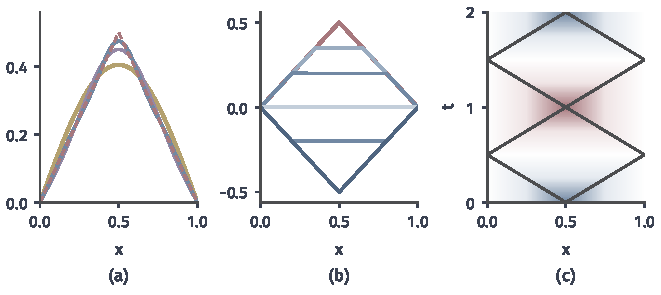
\includegraphics[width=112mm]{figures/06-differential-equations/02-partial-differential-equations/matplotlib/wave-plucked-series/figure.pdf}
  \caption{中点拨起的弦，$L=1$，$c=1$，$u_0=\min\{x,1-x\}$。(a)正弦级数的部分和，黄、紫、蓝分别取到$n=1,3,7$，红色虚线是$u_0$。(b)解的快照，红色是$t=0$，蓝色深浅为$t=0.15,0.3,0.5,0.7,1$，$t=1$时弦完全翻转。(c)时空热图（蓝正红负），深灰折线是在端点反射的特征线，也是折角的轨迹。}
  \label{fig:wave-plucked-series}
\end{BookInlineFigure}

\paragraph{时间因子：振荡与衰减}
同样的空间模式，在第~\ref{chap:diffusion-equations}章的热方程$\partial_tu=\partial_x^{2}u$中，第$n$个模式的时间因子是$\mathrm{e}^{-n^{2}\pi^{2}t}$（$L=1$），在波动方程中是$\cos(n\pi t)$（$c=1$）。图~\ref{fig:wave-heat-mode-factor}并排画出了前三个因子。

热方程的高频模式衰减极快，这就是折角瞬间消失的原因。波动方程的高频模式幅度完全不变，只是振荡得更快。所以波动方程不会平滑初值，初值的高频成分永远留在解里。

\begin{BookInlineFigure}
  \centering
  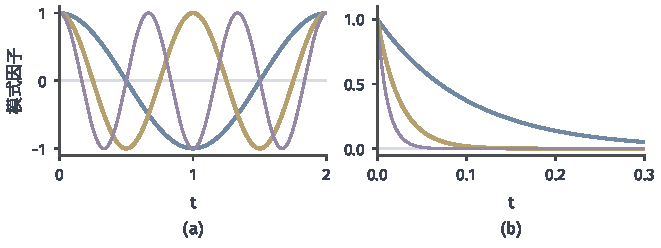
\includegraphics[width=112mm]{figures/06-differential-equations/02-partial-differential-equations/matplotlib/wave-heat-mode-factor/figure.pdf}
  \caption{第$n$个模式的时间因子，$L=1$，蓝、黄、紫依次为$n=1,2,3$。(a)波动方程$\cos(n\pi t)$，$c=1$，幅度不衰减。(b)热方程$\mathrm{e}^{-n^{2}\pi^{2}t}$，模式越高衰减越快（注意时间轴范围不同）。}
  \label{fig:wave-heat-mode-factor}
\end{BookInlineFigure}

\paragraph{离散的模式}
回到式~\eqref{eq:wave-chain}的珠链，看模式如何从有限维走到无限维。设$L=1$，$c=1$，有$N$颗珠子，$h=1/(N+1)$。$\bm{K}$的特征向量正是在格点上取值的$\sin(k\pi x)$，特征值和频率是
\begin{equation}
 \lambda_k=\frac4{h^{2}}\sin^{2}\frac{k\pi h}{2},\qquad \omega_k=\sqrt{\lambda_k}=\frac2h\sin\frac{k\pi h}{2},\qquad k=1,\ldots,N.
 \label{eq:wave-chain-frequencies}
\end{equation}

$N=3$，$h=1/4$时，三个频率和连续弦的$n\pi$比较如下：
\[
 \begin{aligned}
  \text{珠链：}\quad&\omega_1\approx3.06,\quad\omega_2\approx5.66,\quad\omega_3\approx7.39,\\
  \text{连续弦：}\quad&\pi\approx3.14,\quad2\pi\approx6.28,\quad3\pi\approx9.42.
 \end{aligned}
\]
最低的模式已经很准，最高的模式误差最大。图~\ref{fig:wave-discrete-modes}(a)显示珠链的特征向量恰好是连续模式在格点上的采样，(b)显示频率曲线在$N=15$时低端贴合直线$n\pi$，高端向下弯，不能超过$2/h$。这就是第~\ref{sec:wave-problem}节所说类比的失效之处：珠链只有$N$个模式，频率有上限，连续弦的模式无穷多。

\begin{BookInlineFigure}
  \centering
  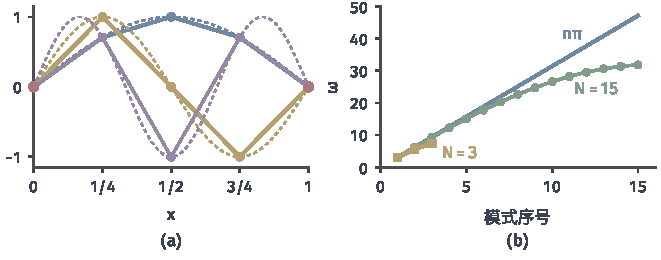
\includegraphics[width=112mm]{figures/06-differential-equations/02-partial-differential-equations/matplotlib/wave-discrete-modes/figure.pdf}
  \caption{珠链和连续弦的模式，$L=1$，$c=1$。(a)$N=3$时的三个特征向量（折线上的点），细虚线是连续模式$\sin(k\pi x)$，红点是固定端。(b)频率随模式序号的变化：蓝线是连续弦$n\pi$，绿线和黄线是$N=15$和$N=3$的珠链。}
  \label{fig:wave-discrete-modes}
\end{BookInlineFigure}
